\documentclass[a4paper,11pt]{scrartcl} 
\usepackage{geometry} 
\geometry{left=2.5cm} \geometry{top=3cm}

\usepackage[utf8]{inputenc} 
\usepackage[ngerman]{babel} 
\usepackage[T1]{fontenc} 
\usepackage{amsmath} 
\usepackage{amssymb} 
\usepackage[onehalfspacing]{setspace} 
\usepackage{graphicx} 
\usepackage{epstopdf} 
\usepackage{csquotes} 
\usepackage{array} 
\usepackage{upgreek} 
\usepackage{float} 
\usepackage{tikz} 
\usepackage[font=small]{caption}
\usepackage[backend=biber, style=chem-angew]{biblatex} 
\addbibresource{Blatt 7.bib} 
\usepackage{tabularx, booktabs, multirow} 
\usepackage{listings}
\usepackage{chemgreek}
\usepackage{chemformula}
\captionsetup{format=plain}
%\usepackage{hyperref}
\usepackage[hidelinks]{hyperref}
\usepackage{svg}
\usepackage{subcaption}
\usepackage{siunitx}
\sisetup{detect-weight=true, detect-family=true,locale=DE,range-phrase={\,bis\,},list-final-separator ={\,\linebreak[0] \text{und}\,},separate-uncertainty=true,per-mode = symbol-or-fraction}

\parindent0pt %Kein Einzug am Anfang von Absätzen
\sloppy %Besserer Blocksatz
%\renewcaptionname{ngerman}{\figurename}{Abb.} 
%\renewcaptionname{ngerman}{\tablename}{Tab.} 
\setkomafont{section}{\normalsize}

\lstset{
    language=Python,
    numbers=left,
    numberstyle=\tiny\color{gray},
    numbersep=8pt,
    stepnumber=1,
    frame=single,
    tabsize=4,
    showstringspaces=false,
    breaklines=true,
    keywordstyle=\color{blue}\bfseries,
    stringstyle=\color{red},
    commentstyle=\color{green!50!black},
    basicstyle=\ttfamily\small,
    literate={ö}{{\"o}}1
             {ä}{{\"a}}1
             {ü}{{\"u}}1
             {ß}{{\ss}}1
}

\title{Blatt 11}
\author{Vincent Kümmerle und Elvis Gnaglo}
\date{\today}

\begin{document}

\maketitle

\section{Erstellen einer Vektorgrafik}
Die Vektorgrafik zur Brechung eines Laserstrahls an einem Prisma wurde mit Inkscape erstellt. Die einzelnen Schritte sind in den folgenden Abbildungen dargestellt.

\begin{figure}[H]
    \centering
    \begin{subfigure}[b]{0.49\textwidth}
        \centering
        \includegraphics[width=\textwidth]{Bilder/Screenshot 2026-01-06 114503.png}
        \caption{Erstellung des Dreiecks mit Polygon-Werkzeug.}
        \label{fig:bild1}
    \end{subfigure}
    \begin{subfigure}[b]{0.49\textwidth}
        \centering
        \includegraphics[width=\textwidth]{Bilder/Screenshot 2026-01-06 115313.png}
        \caption{Erstellung des Laserstrahls.}
        \label{fig:bild2}
    \end{subfigure}
\end{figure}

\begin{figure}[H]
    \centering
    \begin{subfigure}[b]{0.49\textwidth}
        \centering
        \includegraphics[width=\textwidth]{Bilder/Screenshot 2026-01-06 121853.png}
        \caption{Hinzufügen der gebrochenen Strahlen mit dem Bezier-Werkzeug und des Winkels als Text.}
        \label{fig:bild1}
    \end{subfigure}
    \begin{subfigure}[b]{0.49\textwidth}
        \centering
        \includegraphics[width=\textwidth]{Bilder/Screenshot 2026-01-06 123015.png}
        \caption{Erstellung des Einfalls- und Ausfallslots.}
        \label{fig:bild2}
    \end{subfigure}
\end{figure}
Im letzten Schritt wurde die Seitengröße an den Rahmen um alle Objekte angepasst und die Grafik als PDF exportiert.
\begin{figure}[H]
    \centering
    \includegraphics[width=0.9\textwidth]{Bilder/Screenshot 2026-01-06 131836.png}    
    \caption{Anpassung der Seitengröße an den Rahmen um alle Objekte.} 
\end{figure}

Die erstellte Vektorgrafik ist in Abbildung \ref{fig:Prisma} dargestellt.
Sie zeigt die Brechung eines monochromatischen Laserstrahls an einem Prisma mit dem Einfallswinkel $\alpha$, dem Einfalls- und Ausfallslot sowie den gebrochenen Strahlen im Prisma.
\begin{figure}[H]
    \centering
    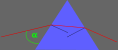
\includegraphics[width=0.8\textwidth]{Bilder/Lichtbrechung.pdf}    
    \caption{Strahlengang eines monochromatischen Laserstrahls an einem Prisma mit Einfallswinkel $\alpha$.}
    \label{fig:Prisma} 
\end{figure}


\section{Lineare Algebra mit NumPy: Fibonacci-Folge}
Das vorliegende Python-Skript untersucht das Konvergenzverhalten des Verhältnisses aufeinanderfolgender Fibonacci-Zahlen $a_n / a_{n-1}$ mithilfe von Matrix-Vektor-Multiplikationen und einer Eigenwertanalyse.\\
Zunächst werden die Anfangswerte der Fibonacci-Folge als Vektor $v = (1, 1)^T$ initialisiert, was den Startwerten $a_2 = 1$ und $a_1 = 1$ entspricht. Die Iterationsvorschrift wird durch die Matrix $M$ definiert:
\begin{equation}
    M = \begin{pmatrix} 1 & 1 \\ 1 & 0 \end{pmatrix}
\end{equation}

Die resultierenden Verhältnisse werden graphisch als diskrete Punkte über der Anzahl der Iterationen aufgetragen.\\
Im zweiten Teil des Skripts wird das Verhalten der Folge durch die spektralen Eigenschaften der Matrix $M$ erklärt. Mithilfe der Funktion \texttt{np.linalg.eig} werden die Eigenwerte und Eigenvektoren von $M$ numerisch bestimmt.\\
Da $M$ symmetrisch ist, existieren reelle Eigenwerte. Diese werden nach ihrem Betrag sortiert, um den dominanten Eigenwert $\lambda_1$ zu identifizieren. Theoretisch ergeben sich die Eigenwerte aus dem charakteristischen Polynom $\lambda^2 - \lambda - 1 = 0$ zu:
\begin{equation}
    \lambda_{1,2} = \frac{1 \pm \sqrt{5}}{2}
\end{equation}
Der dominante Eigenwert ist der Goldene Schnitt $\lambda_1 \approx 1.618$. 

Das Skript vergleicht die iterative Lösung mit diesem theoretischen Grenzwert. Dazu wird eine konstante Linie (rote gestrichelte Linie) auf Höhe von $\lambda_1$ in den Plot eingezeichnet.\\
Die graphische Auswertung zeigt, dass das Verhältnis $a_n / a_{n-1}$ sehr schnell gegen den dominanten Eigenwert $\lambda_1$ konvergiert. Anfangs sind Oszillationen sichtbar, die jedoch rasch abklingen, da der Einfluss des betragsmäßig kleineren Eigenwertes $|\lambda_2| < 1$ mit $n \to \infty$ exponentiell verschwindet.\\
\begin{lstlisting}
import numpy as np
import matplotlib.pyplot as plt

# Part 1
v = np.array([1.0, 1.0])
M = np.array([[1, 1], 
              [1, 0]])

ratios = []
n_values = range(50)

for i in range(50):
   current_ratio = v[0] / v[1]
   ratios.append(current_ratio)
   v = M @ v

plt.figure(figsize=(10, 6))
plt.plot(n_values, ratios, linestyle="none", marker="o", label="Numerisches Verhältnis $a_n/a_{n-1}$", markersize=4)


# Part 2
# Berechnung der Eigenwerte und Eigenvektoren
eigenvalues, eigenvectors = np.linalg.eig(M)

# Sortierung nach dem größten Eigenwert
idx = np.argsort(np.abs(eigenvalues))[::-1]
lambdas = eigenvalues[idx]

print(f"Die Eigenwerte von M sind: {lambdas}")
print(f"Dominanter Eigenwert (lambda_1): {lambdas[0]}")

# Approximation:
approx_ratios = [lambdas[0]] * len(n_values)

# Plotten der Approximation
plt.plot(n_values, approx_ratios, color='red', linestyle='--', label=f"Approximation ($\\lambda_1 \\approx {lambdas[0]:.4f}$)")


plt.title("Konvergenz des Verhältnisses von Fibonacci-Zahlen")
plt.xlabel("Iteration n")
plt.ylabel("Verhältnis $a_n / a_{n-1}$")
plt.legend()
plt.grid(True, which="both", linestyle='--', alpha=0.7)
plt.savefig('fibonacci.pdf')
plt.show()
\end{lstlisting}

\begin{figure}[H]
    \centering
    \includegraphics[width=1\textwidth]{Bilder/fibonacci.pdf}    
    \caption{Die geplotteten Verhältnisse der Fibonacci Folge mit der berechneten Approximation.} 
\end{figure}
\newpage
\section{Quicksort-Algorithmus}
\begin{lstlisting}
    def quick_sort(arr):
    # Basisfall: Die Liste ist leer ist oder hat nur ein Element
    if len(arr) <= 1:
        return arr

    # 1. Wahl des Pivot-Elements (mittleres Element)
    pivot = arr[len(arr) // 2]

    # 2. Aufteilen der Liste in drei Teile
    # Elemente < Pivot
    left = [x for x in arr if x < pivot]
    
    # Elemente = Pivot (Duplikate)
    middle = [x for x in arr if x == pivot]
    
    # Elemente > Pivot
    right = [x for x in arr if x > pivot]

    # 3. Rekursiver Aufruf und Zusammenfügen der Ergebnisse
    return quick_sort(left) + middle + quick_sort(right)

#Beispiel
b_liste = [3, 6, 8, 10, 1, 2, 1, 90, 4, 9, 0, -1]
s_liste = quick_sort(b_liste)

print(f"Original: {b_liste}")
print(f"Sortiert: {s_liste}")
\end{lstlisting}


\end{document}